% vim: set tw=78 sts=2 sw=2 ts=8 aw et ai:

\chapter{Use Case Application}
\label{chapter:app}

Developing OpenFlow features for Open vSwitch is only part of the process. Application controllers need to make
use of these features to implement higher level functionalities. We did this by writing a simple learning
switch controller using the Ryu\cite{ryu} SDN framework. Is uses Snort and OpenFlow bundles to act like an Intrusion
Prevention System and block malicious nodes in a local network.

\begin{figure}[h]
\begin{center}
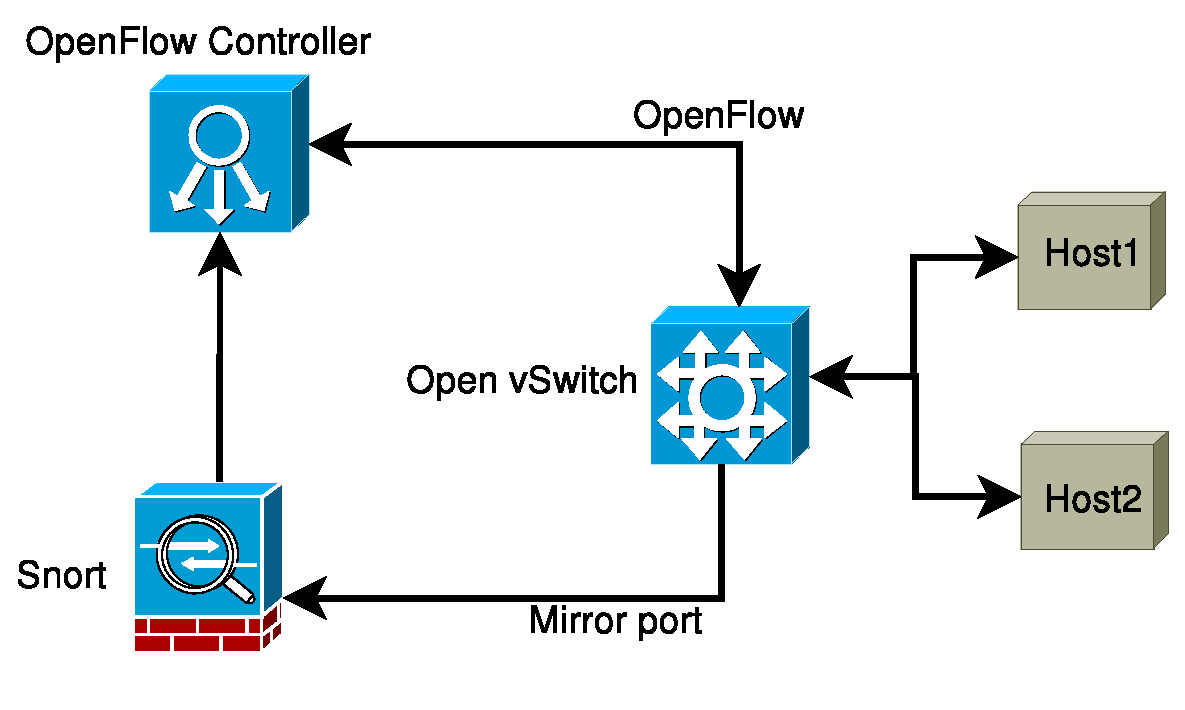
\includegraphics[scale=0.5]{src/img/test-app.eps}
\end{center}
\caption{Test Application}
\label{fig:testapp}
\end{figure}

Ryu has support\footnote{\url{https://github.com/osrg/ryu/wiki/Snort-Integration}} for receiving Snort notifications and acting upon them.
However, we wanted to also test the bundles feature that we implemented so we designed our own controller. The two hosts
are KVM virtual machines, connected to Open vSwitch, instead of the usual Linux bridge. Figure~\ref{fig:testapp} shows and
overview of the application. A third port is used to mirror all the packets going through the switch. Snort is monitoring
this port and writing the alerts in a simple to parse CSV log.

The Ryu controller has the main function of being a learning switch. It stores a mapping of the ports corresponding to each host address
and only floods all ports when no mapping exists. The switch is configured to send packets to
the controller when there are no flows matching. The switch will check if the source of the
packet is blacklisted and will block the port if it is. Otherwise, new flows will be inserted
to allow future packets to be forwarded.

Another thread is watching the Snort log file for changes. When new alerts are found, the source
of the alert is added to a list of blacklisted hosts. Flows that will block this host can then
be sent to one or more switches.

The OpenFlow bundles can be used here to direct traffic away from the malicious nodes in a network.
The controller can be programmed to send multiple flows to several controllers and, at the same time,
also block the source node. If this node is providing an important service, the presented solution could
be used to implement high availability in the case when the host gets compromised.
  